%%%%%%%%%%%%%%%%%%%%%%%%%%%%%%%%%% Beamer-Presentation 2022 %%%%%%%%%%%%%%%%%%%%%%%%%%%%%%%%%
	\documentclass[12pt]{beamer}
%%%%%%%%%%%%%%%%%%%%%%%%%%%%%%%%%%%%%%%%%%%%%%%%%%%%%%%%%%%%%%%%%%%%%%%%%%%%%%%%%%%%%%
	%\usepackage{pgfpages}
	%\pgfpagesuselayout{4 on 1}[a4paper, border shrink=5mm, landscape]
	%==================================== Preamble ==========================================
	%-------------------------------- preamble.tex ------------------------------------------
\graphicspath{{gfx/}}

%=================================== Packages ==============================================
\usepackage[T1]{fontenc}
\usepackage{ragged2e}\justifying
\usepackage{txfonts}
\usepackage{booktabs}
\usepackage{natbib}
\usepackage{bibentry}
\usepackage{appendixnumberbeamer}
\usepackage{pifont}
\usepackage{fontawesome}
\usepackage{textpos}
\usepackage{media9}
\usepackage{tikz}
%\usepackage{multirow}
\usepackage{multicol}
%\usepackage{amsmath}
\usepackage[compat=1.1.0]{tikz-feynman}

%=================================== Themes ==============================================
\usetheme{EastLansing}
\useoutertheme[footline=authortitle,subsection=false]{miniframes} % Alternatively: miniframes, infolines, split
% \useinnertheme{circles}
\usefonttheme{serif}
%========================= Beamer color/font/template ==================================== 
\definecolor{UBCblue}{rgb}{0.04706, 0.13725, 0.26667} % UBC Blue (primary)
\definecolor{UBCgrey}{rgb}{0.3686, 0.5255, 0.6235} % UBC Grey (secondary)
\definecolor{sviolet}{rgb}{0.3, 0.08, 0.8235}
% % ===============================================================

% Override palette coloring with secondary

% \setbeamercolor{palette primary}{bg=red,fg=white}
% \setbeamercolor{palette secondary}{bg=violet,fg=white}
% \setbeamercolor{palette tertiary}{bg=sviolet,fg=white}
\setbeamercolor{section in head/foot}{bg=sviolet,fg=white}
% \setbeamercolor{palette quaternary}{bg=red,fg=white}
\setbeamercolor{subsection in head/foot}{bg=sviolet,fg=white}

% \setbeamercolor{structure}{fg=UBCblue} % itemize, enumerate, etc

\setbeamercolor{section in toc}{fg=sviolet} % TOC sections
% color of title and frame title 
\setbeamercolor{title}{bg=sviolet,fg=white}
\setbeamercolor{frametitle}{fg=UBCblue}

\setbeamercolor{author}{fg=blue}
\setbeamercolor{institute}{fg=blue} 
\setbeamercolor{author in head/foot}{bg=green!50!blue}
\setbeamercolor{title in head/foot}{bg=blue!70!white}
\setbeamercolor{frametitle}{fg=sviolet,bg=blue!10!white}
% ===============================================================

 
\setbeamersize{text margin left=12mm, text margin right=12mm} 
\setbeamertemplate{frametitle}[default][left, leftskip=5mm] 
\setbeamertemplate{frametitle continuation}{\frametitle{References}}
\setbeamertemplate{bibliography item}[text] 
\setbeamertemplate{page number in head/foot}[appendixframenumber]
\setbeamertemplate{navigation symbols}{} %hides navigation buttons at bottom
% \setbeamertemplate{headline}{} %hides navigation bar at top


\setbeamercovered{transparent}
% \setbeamercovered{invisible}

\setbeamertemplate{footline}{%
	\leavevmode\bfseries 	
	\begin{beamercolorbox}[wd=0.5\paperwidth, ht=7pt, dp=2.5pt, center]{author in head/foot}
	\insertshortauthor%~(\insertshortinstitute)
	\end{beamercolorbox}%
	\begin{beamercolorbox}[wd=0.5\paperwidth, ht=7pt, dp=2.5pt, center]{title in head/foot}
	\insertshorttitle
	\end{beamercolorbox}%
}

\setbeamertemplate{frametitle}[default][left, leftskip=2mm] 
\setbeamertemplate{frametitle continuation}{\frametitle{References}}
% \setbeamerfont{frametitle}{series=\bfseries}
\setbeamertemplate{frametitle}{%	
	\nointerlineskip		
	\begin{beamercolorbox}[wd=\paperwidth, ht=5.4mm, dp=2.5mm]{frametitle}
	\hskip3mm
	\insertframetitle	
	\end{beamercolorbox}%   
}
\addtobeamertemplate{frametitle}{}{%
	\begin{textblock*}{100mm}(0.95\linewidth, -7.7mm)
		
\includegraphics[height=7.4mm, width=7.4mm]{logo1}	
		
\includegraphics[height=7.4mm, width=7.4mm]{logo2}
	\end{textblock*}
}
%=================================== Others ==============================================
\setlength{\parskip}{5pt}

\let\oldbib\bibentry
\renewcommand{\bibentry}[1]{{\tiny[\oldbib{#1}]}}
%=========================End Preamble======================================
	%=============================== Title information ======================================
	\title[Measurment of Branching Franction]{Measurment of Branching Franction of $B^{-}\to D^{0} \pi^{-}\pi^{+}\pi^{-}$}
	%\subtitle{Write the subtitle}

	\author[Shubhajit Sana \hspace{4 pt} (Guide: Prof. J. Libby)]{Shubhajit Sana\\  Roll: PH18B004\\ Guide: Prof. James F. Libby\\[5mm] 
	
\includegraphics[scale=0.04]{logo1}
	\hspace{2 cm}
	
\includegraphics[width=1.8cm]{logo2}
	}

	\institute[IIT Madras]{Department of Physics,\\ Indian Institute of Technology Madras, \\ Chennai 600036, India}

	%\date[\tiny \today]{\scriptsize \today}
	\date{November 22, 2022}

	%\titlegraphic{\includegraphics[scale=0.08]{logo}}
	% \logo{\includegraphics[scale=0.04]{logo}}

	%=================================== Main body========================================
	\begin{document}

	%% References	
	\bibliographystyle{APA-noTitle}
	\nobibliography{mybib}	

	%% Title frame	
	\begin{frame}[plain, noframenumbering]
	\maketitle
	\end{frame}	

	%--------------------------------------------------------------------------
	% \section[Outline]{}
	%-------------------------------------------------------------------------

	%% TOC
	\begin{frame}{Outline}
		\tableofcontents	
	\end{frame}
	%Showing Outline before every section
	% \AtBeginSection[]{
	% \begin{frame}{Outline}
	% 	\tableofcontents[currentsection]	
	% \end{frame}
	% }
%--------------------------------------------------------------------------
\section[SuperKEKB]{SuperKEKB Accelerator}
%--------------------------------------------------------------------------
	\begin{frame}[t]{SuperKEKB accelerator}
		\begin{columns}
			\column{0.5\textwidth}
			
			\begin{itemize}
				\begin{scriptsize}
					\item Super KEKB: 4 GeV $ e^{+} $ and 7 GeV $ e^{-} $ asymmetric collider at KEK, Japan.
					\item 3 km circumference and 41 mrad crossing angle. 
					\item The center-of-mass energy is close to the mass of $ \Upsilon (4S) $, which decays later to $ B\overline{B} $ pair.
					\item A 30-fold increase in Luminosity over Belle, $ L = 6 x 10^{35}$cm$^{-2}$s$^{-1} $.
					\item Uses the nano-beam scheme (minimization of vertical beta function); hence doubled current.
					\item Better performance and can tolerate the much higher level of beam-related backgrounds due to the increase in instantaneous luminosity.
					\item \textbf{Belle II detector} is at the interaction point.
				\end{scriptsize}
			\end{itemize}
			
			\column{0.5\textwidth}
			\begin{figure}
				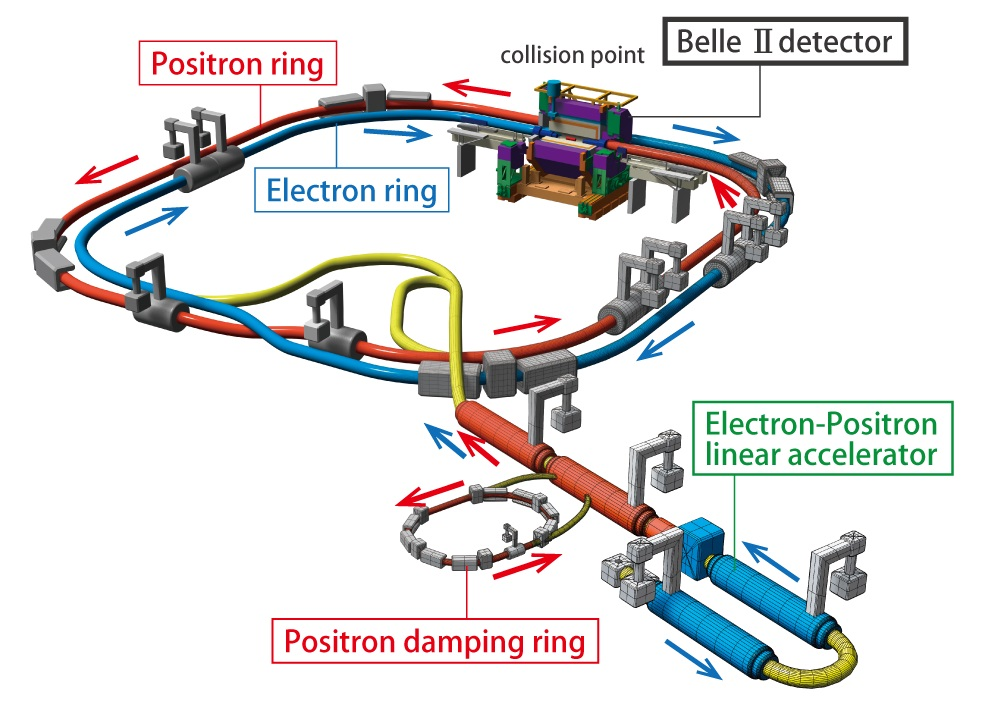
\includegraphics[height = 5 cm, width = 6cm]{skekb.jpg}
				\caption{SuperKEKB accelerator}
			\end{figure}
			
		\end{columns}
		
	\end{frame}
%--------------------------------------------------------------------------
\section[Belle II]{Belle II detector}
%--------------------------------------------------------------------------
	\begin{frame}[t]{Belle II detector}
		\vspace{-0.1 in}
		\begin{columns}
			\column{0.5\textwidth}
			\begin{itemize}
				\begin{scriptsize}
					\item Vertex detector (PXD$ + $SVD): two layers of pixel detector and four layers of SVD to determine $ B $ meson decay vertices.
					\item Central drift chamber (CDC): A large gaseous detector that acts as the principal tracking
					device.
					\item Aerogel Ring Imaging Cherenkov Counter (ARICH): Used for particle identification, mainly to distinguish between pions and kaons.
					\item Time-of-Propagation Counters (TOP): Cerenkov radiation totally internally reflected within quartz bars for particle identification.
					\item Electromagnetic calorimeter (ECAL): Detects photons and measures their energy
					and position with thallium-doped caesium iodide crystals.
					
					
				\end{scriptsize}
			\end{itemize}
			
			\column{0.5\textwidth}
			
			\begin{figure}
				\vspace{-0.3 in}
				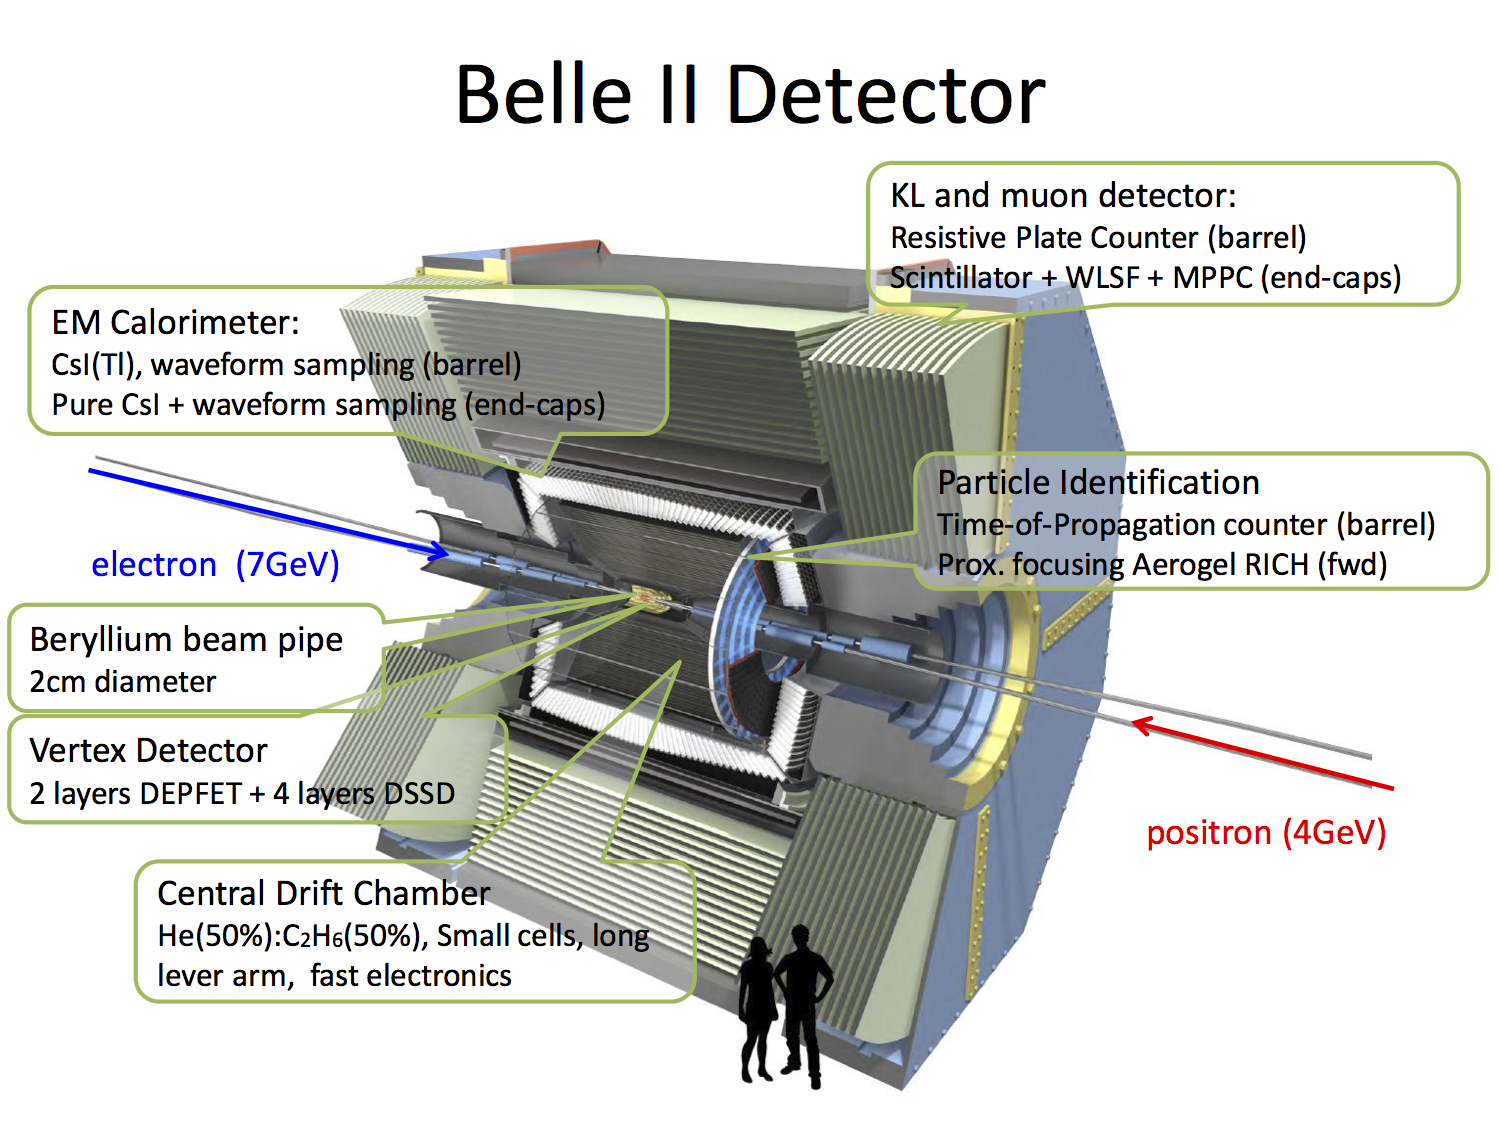
\includegraphics[height = 5cm,width = 6cm]{Belle2.png}
			\end{figure}
			\vspace{-0.22 in}
			\begin{scriptsize}
				\begin{itemize}
					\item K-Long and muon detector (KLM): Detects muons and long-lived neutral kaons, and distinguishes between them using scintillators along with RPCs.
					\item Superconducting Solenoid : Provides a homogeneous magnetic field of 1.5T along the	beam axis.
				\end{itemize}
			\end{scriptsize}
		\end{columns}
		
	\end{frame}

%--------------------------------------------------------------------------
\section[FEI]{Full Event Interpretation}
%--------------------------------------------------------------------------
	\begin{frame}[t]{Full Event Interpretation}
		\begin{scriptsize}
			\begin{columns}
				\column{0.5\textwidth}
				\begin{itemize}
					\begin{scriptsize}
						\item Implement tagging, where one B referred to as $B_{tag}$ is exclusively reconstructed using hadronic or semi-leptonic modes.
						\item The remaining tracks and clusters	are then attributed to $B_{sig}$, on which the search or measurement of a particular decay is done.
						\item Any missing energy is attributed to the $B_{sig}$.
					\end{scriptsize}
				\end{itemize}
				
				\column{0.5\textwidth}
				\vspace{-0.6cm}
				\begin{figure}
					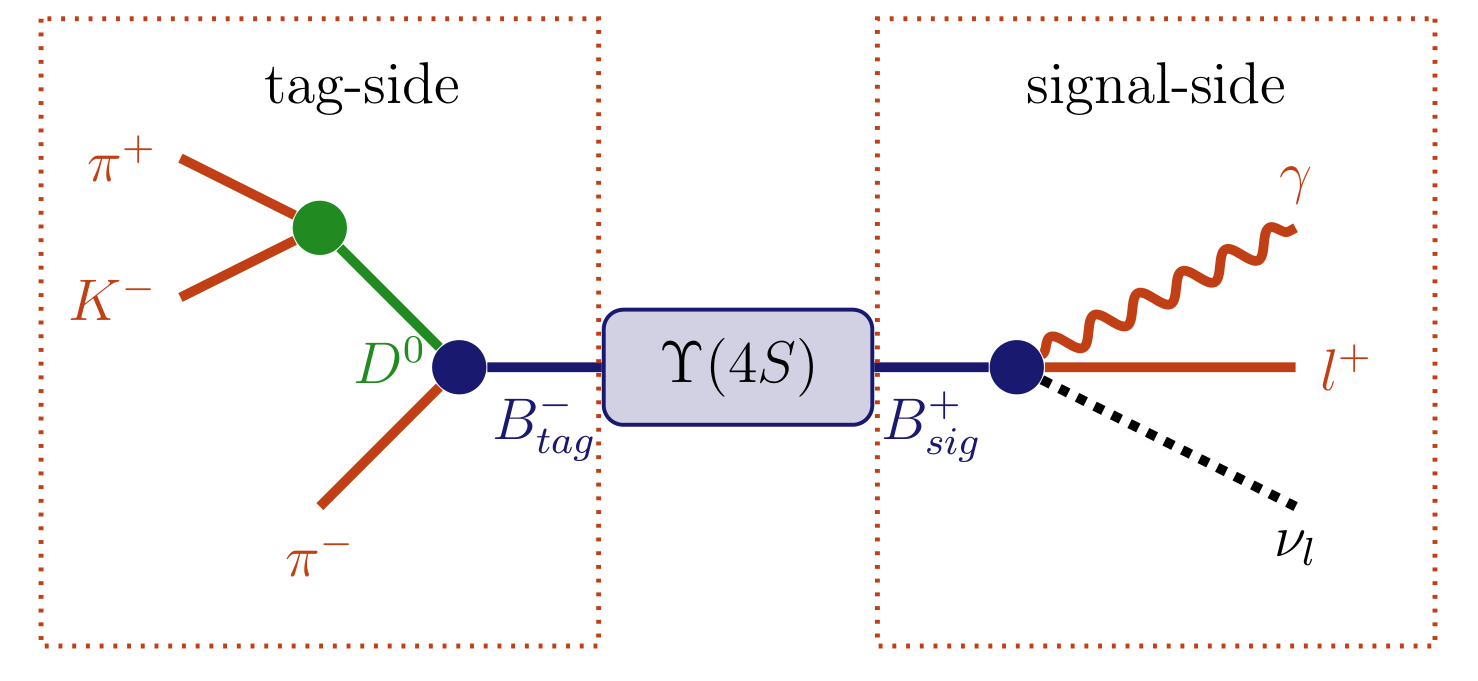
\includegraphics[height = 4 cm, width = 6cm]{tag.png}
				\end{figure}
			\end{columns}
			\vspace{-0.1cm}%\hspace{2.5cm}
			\begin{figure}
				%\hspace{2.5cm}
				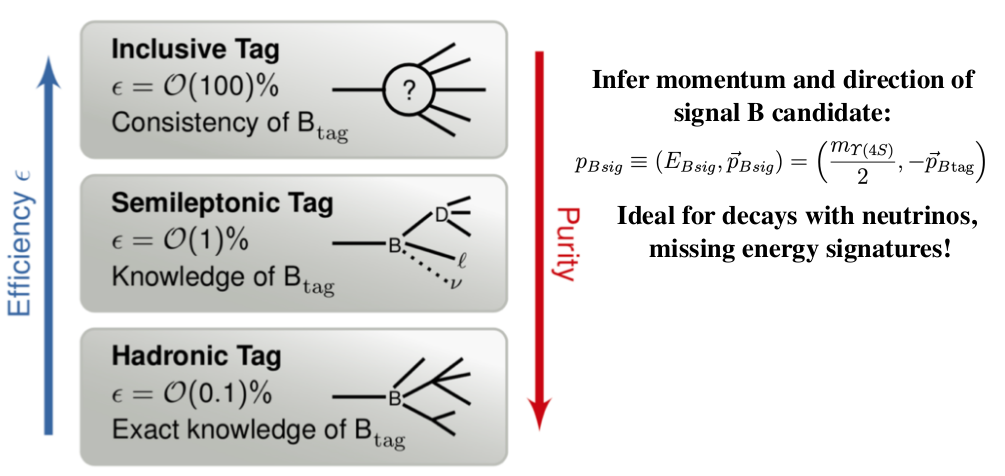
\includegraphics[scale=0.2]{infer.png}
			\end{figure}
		\end{scriptsize}
	\end{frame}
	\begin{frame}[t]{Full Event Interpretation}
		\fontsize{10pt}{10pt}\selectfont
		%\begin{scriptsize}
		\begin{columns}
			\column{0.5\textwidth}
			\begin{itemize}
				%\begin{scriptsize}
				\item Final-state particle candidates are selected and corresponding classification methods are trained using the detector information.
				\item Intermediate particle candidates are reconstructed and a multivariate classifier is trained for each employed decay channel.
				\item Employs over 200 Boosted Decision Trees to reconstruct more than 10000 B decay modes.
				%\end{scriptsize}
			\end{itemize}
			
			
			\column{0.5\textwidth}
			\begin{figure}
				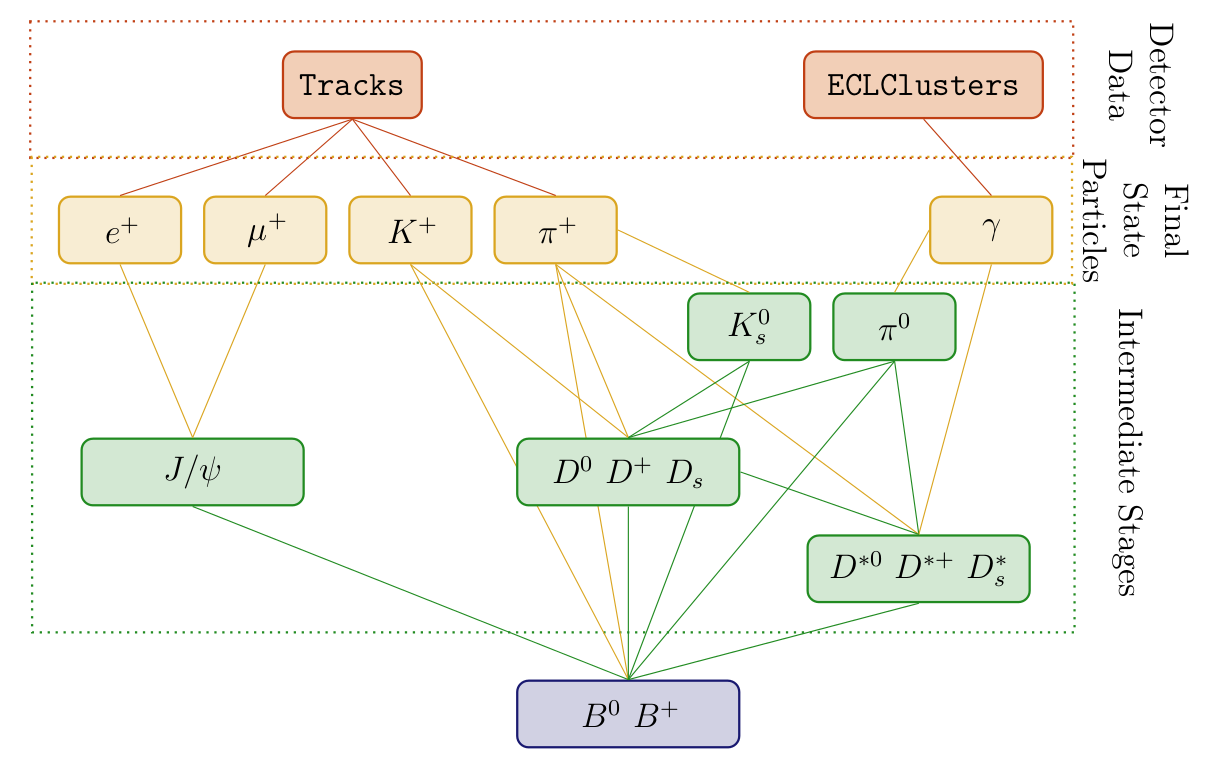
\includegraphics[height = 5 cm, width = 6cm]{hierarchy.png}
				\caption{MVC algorithm with Hierarchal approach}
			\end{figure}
			
		\end{columns}
		%\end{scriptsize}
	\end{frame}

	\begin{frame}[t]{Boosted Decesion Tree}
	%\fontsize{10pt}{10pt}\selectfont
	\begin{scriptsize}
		\begin{itemize}
			\item Boosted Decision Trees (BDTs) are a specific type of a machine learning model used for classification tasks.
			\item The name decision tree refers to the general structure: the classification is done with a series of “decisions”.
			\item Decisions are logical operations (like “>”, “<”, “=”, etc.) on the input variables of each data point, by the outcome of which the data points are separated into groups.
			\item The word boosted refers to the specific way the tree is formed: gradient boosting. Gradient boosting means, that a final tree is made by combining a series of smaller trees of a fixed depth.
			\item The BDT is a supervised machine learning method, i.e. it needs to be trained on a dataset where we know the true class that we are trying to predict (this variable is called the target variable).
		\end{itemize}
	\end{scriptsize}
	\begin{columns}
		\hspace{0.5cm}
		\column{0.5\textwidth}
			\begin{scriptsize}
				\vspace{-0.5cm}
		\begin{itemize}
			\item FastBDT is the fastest contestant for small models (depth of the trees <5 and number of trees <300), whereas XGBoost has a slightly better scaling behaviour for large models.
			\item Used in FEI and to reject continuum background. 
		\end{itemize}
		\end{scriptsize}
		\column{0.5\textwidth}
		\vspace{-0.4cm}
		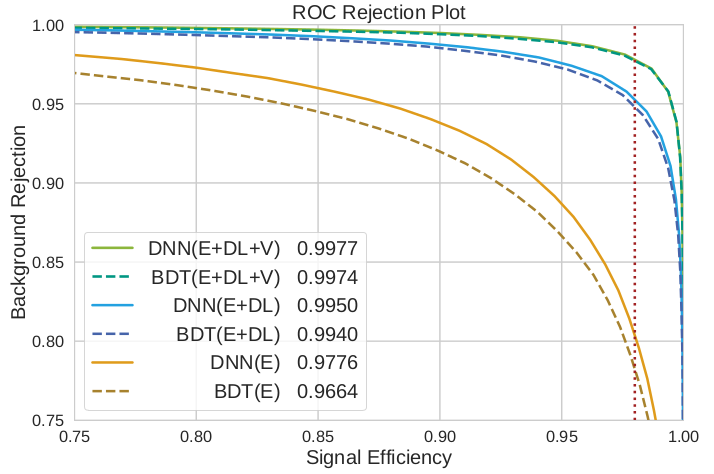
\includegraphics[height = 3.8 cm, width = 6cm]{bdt.png}
		
	\end{columns}
	\end{frame}

	%\begin{frame}[t]{Belle II detector}
	%\fontsize{10pt}{10pt}\selectfont
		
	%\end{frame}

	%\begin{frame}[t]{Belle II detector}
	%\fontsize{10pt}{10pt}\selectfont
		
	%\end{frame}
%--------------------------------------------------------------------------
\section{Motivation}
%--------------------------------------------------------------------------
	\begin{frame}[t]{Motivation}
		\begin{scriptsize}
			\begin{itemize}
				\item Inclusive and exclusive $b \to ul\nu$ and $b \to cl\nu$ transitions are crucial for the determination of the CKM matrix elements $\vert V_{ub} \vert$ and $\vert V_{cb} \vert$.\\
				\begin{center}
					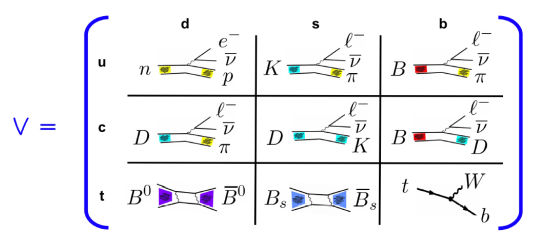
\includegraphics[scale=0.25]{v}
				\end{center}
				\item FEI is a powerful technique to reconstruct such decays with missing energy.
				\item Tag decays include high branching fraction decays like $B^{-}\to D^{0} \pi^{-}\pi^{+}\pi^{-}$.
				\begin{center}
					\footnotesize
					\fcolorbox{red}{white}{BF=(5.6$\pm$ 2.1) $\times$ $10^{-3}$}
				\end{center}
			\item However it is not well simulated in MC because of the large uncertainity on the branching fraction.
			\item Goal is to improve the accuracy of the branching fraction measurement of $B^{-}\to D^{0} \pi^{-}\pi^{+}\pi^{-}$.
			\end{itemize}
		\end{scriptsize}
	\end{frame}
%--------------------------------------------------------------------------
\section[Analysis]{Analysis}
%--------------------------------------------------------------------------
\begin{frame}[t]{Cuts}
	\begin{scriptsize}
	\begin{itemize}
		% \item The BF measurements are based on the following equations:
		% $$
		% 	\mathcal{B}(\mathrm{B}^{+} \rightarrow \bar{\mathrm{D}}^{0}\pi^{+}\pi^{-}\pi^{+}) 
		% 	= \frac{N_{sig}}{2 \cdot \varepsilon \cdot \mathcal{L} \cdot \sigma_{B^+B^-} \cdot 
		% 	\mathcal{B}(\bar{\rm D}^0 \rightarrow K^{+} \pi^{-})}
		% $$
		\item Data Set: MC15ri$\_$a inclusive MC (200 $fb^{-1}$)
		\item \textbf{Object selection:}
		\begin{itemize}
			\begin{scriptsize}
			\item Transverse impact parameter $\vert$d0$\vert$ < 0.2 cm.%eliminate poorly-reconstructed tracks that do not originate from the IP region
			\item Longitudinal impact parameter $\vert$z0$\vert$ < 1 cm.%eliminate poorly-reconstructed tracks that do not originate from the IP region
			\item Polar angle $\to$ 0 < $\theta$ < 126.87: $\cos\theta$ >= -0.6% remove backward tracks (outside the PID sub-detectors)
			\end{scriptsize}
		\end{itemize}
		\item Selection on kinematic variables:
		\begin{itemize}
			\begin{scriptsize}
			\item Mass of $D^{0}$ meson: 1.84 < M < 1.89 GeV/c$ ^{2} $
			\item Beam constrained mass ($M_{bc}$) > 5.27 GeV/c$ ^{2} $, defined as $ M_{\rm bc} = \sqrt{E_{\rm beam}^{2} - (\Sigma \overrightarrow{p_{i}})^{2}}$
			\item Beam-energy Difference $ \vert \Delta E \vert <$ 0.15 GeV, defined as $ \Delta E = \Sigma E_{i} - E_{\rm beam} $.
			\end{scriptsize}			
		\end{itemize}
		
	\end{itemize}
	\end{scriptsize}
\end{frame}

\begin{frame}[t]{M$_{bc}$}
\begin{scriptsize}
			\begin{columns}
		\column{0.5\textwidth}
		\begin{figure}
			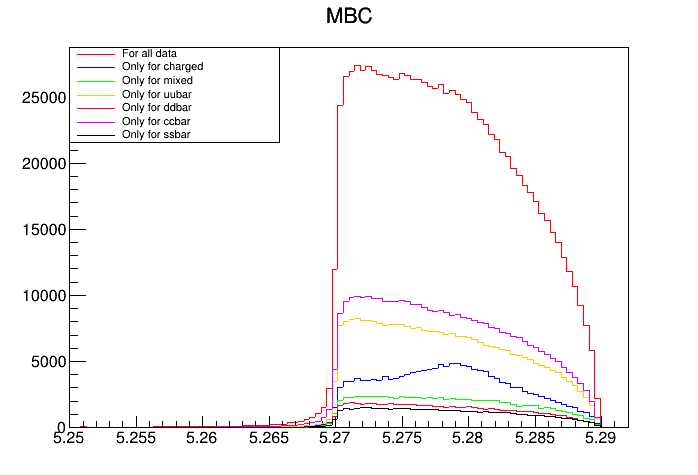
\includegraphics[height = 5 cm, width = 6cm]{Mbc_all.png}
			\caption{Plotting M$_{bc}$ for different profile}
		\end{figure}
		
		\column{0.5\textwidth}
		\begin{figure}
			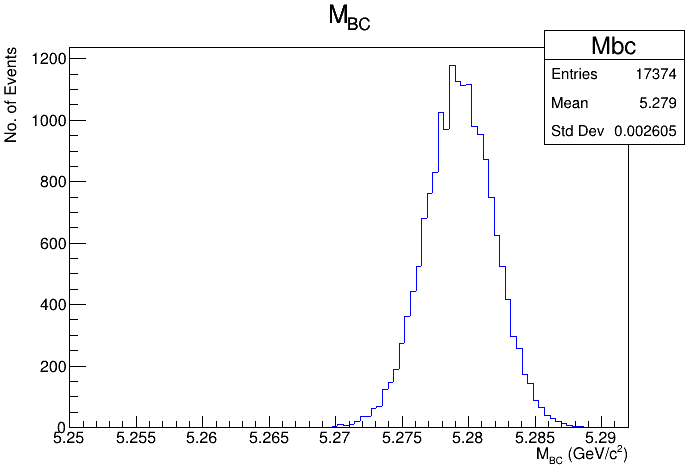
\includegraphics[height = 5 cm, width = 6cm]{Mbc_sig.png}
			\caption{Plotting M$_{bc}$ for Truth Matched(TM) events}
		\end{figure}
		
	\end{columns}
\end{scriptsize}
\end{frame}

\begin{frame}[t]{Delta E}
	\begin{scriptsize}
		\begin{columns}
			\column{0.5\textwidth}
			\begin{figure}
				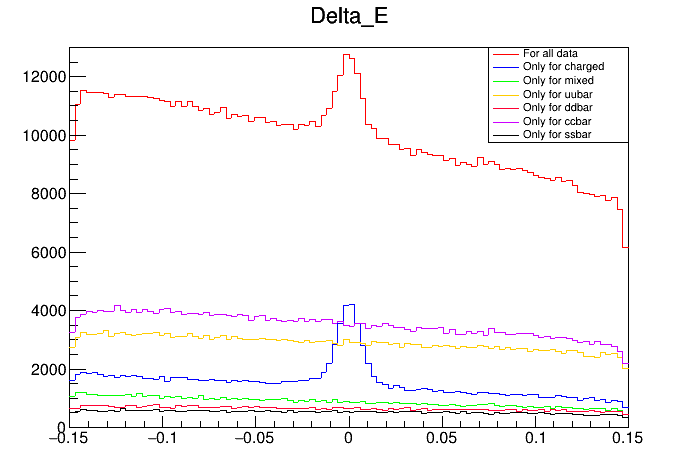
\includegraphics[height = 5 cm, width = 6cm]{de_all.png}
				\caption{Plotting $\bigtriangleup$E for different profile}
			\end{figure}
			
			\column{0.5\textwidth}
			\begin{figure}
				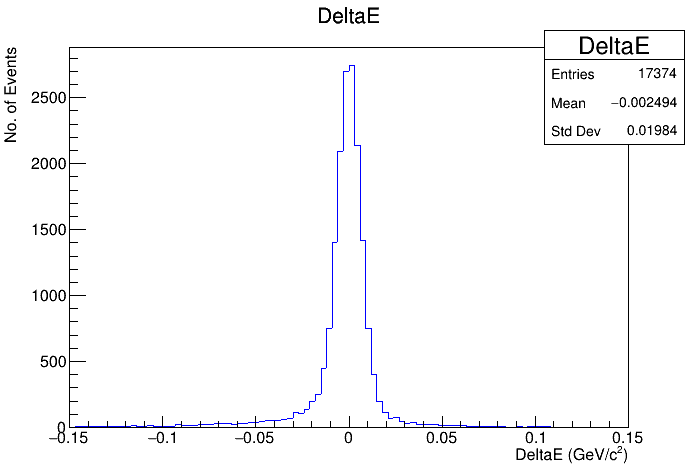
\includegraphics[height = 5 cm, width = 6cm]{de_sig.png}
				\caption{Plotting $\bigtriangleup$E for Truth Matched(TM) events}
			\end{figure}
			
		\end{columns}
	\end{scriptsize}
\end{frame}

\begin{frame}{}                                                                           
	\begin{figure}
		% \centering
		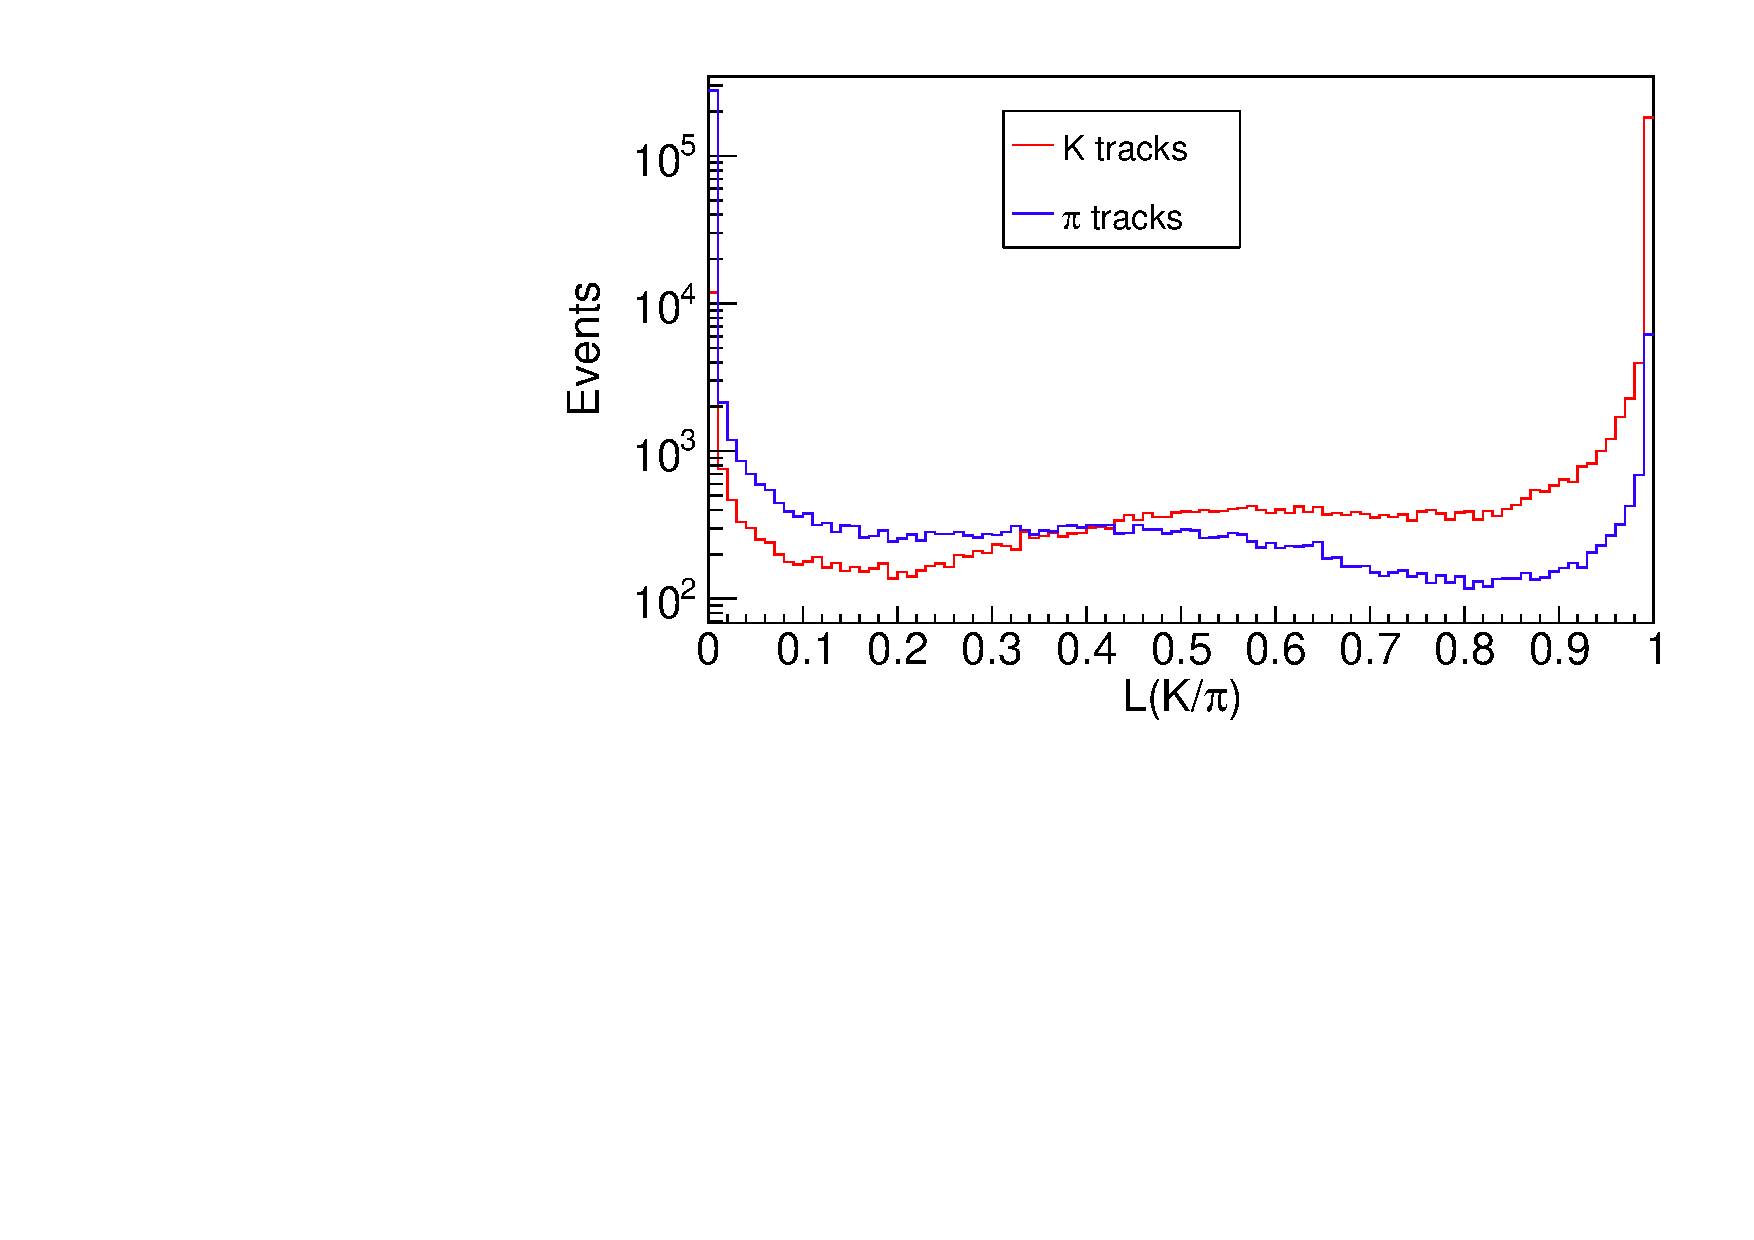
\includegraphics{PID_bin_kaon_pion.pdf}
		% \caption{Distribution of $\mathcal{L}(K \mid \pi)$ for charged kaon and pion tracks in the signal MC sample}
		% \label{fig:binary_pid_kpi}
	\end{figure}
\end{frame}

\begin{frame}{}                                                                           
	\begin{figure}
		% \centering
		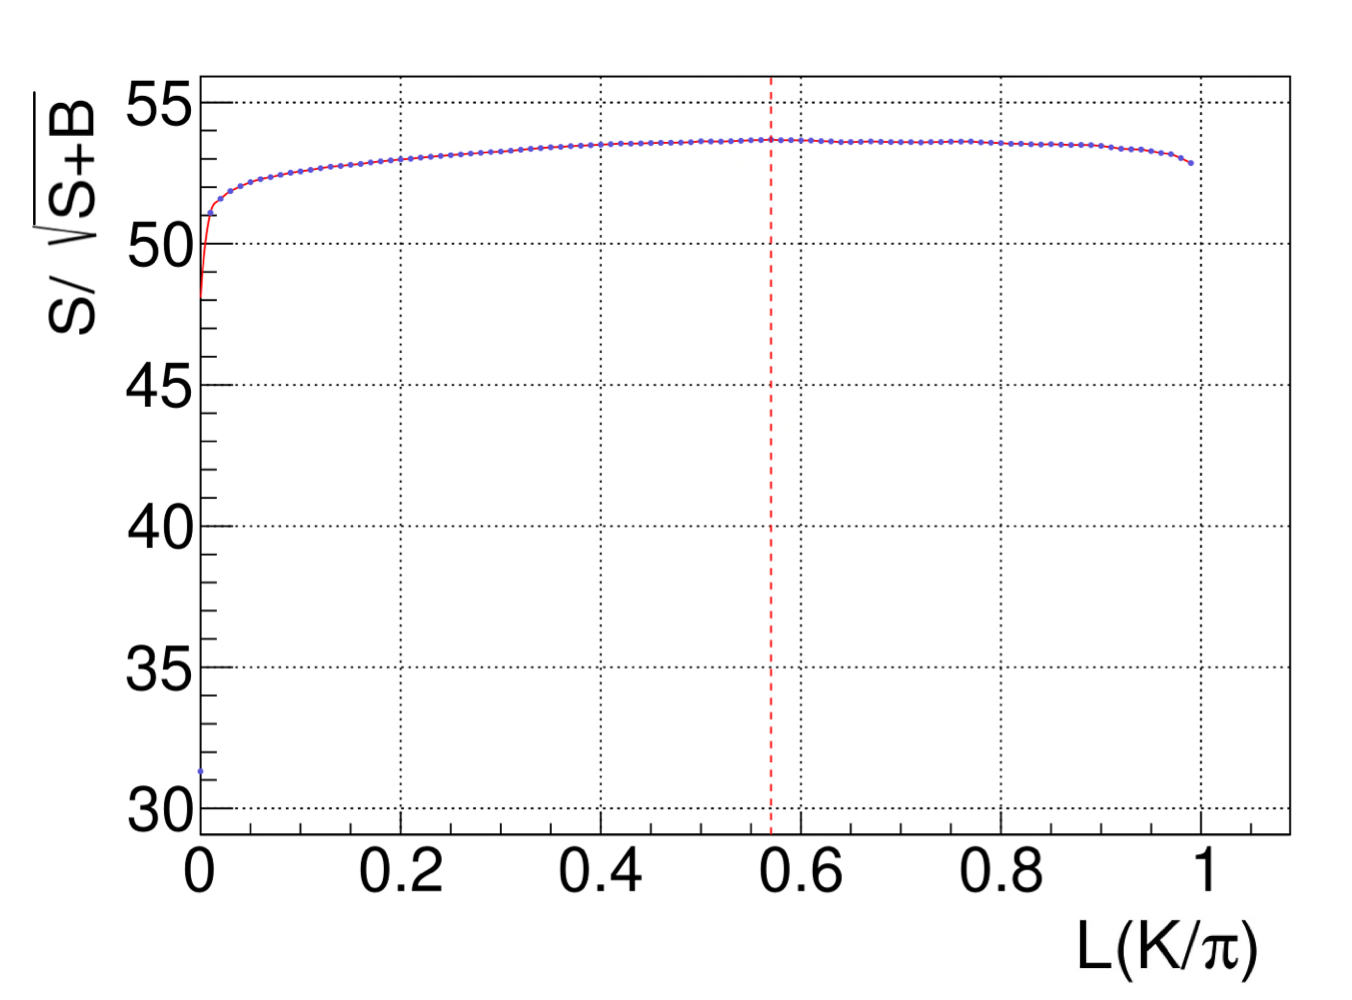
\includegraphics{fom_plot_kid_thesis_channel_07_266_29.png}
		% \caption{Distribution of $S/\sqrt{S+B}$ for PID selection optimization for kaon tracks originating from $\bar{\mathrm{D}}^{0}$}
		% \label{fig:binary_pid_fom}
	\end{figure}
\end{frame}

\begin{frame}{}                                                                           

\end{frame}

\begin{frame}{}                                                                           

\end{frame}

\begin{frame}{}                                                                           

\end{frame}

\begin{frame}{}                                                                           

\end{frame}

































\begin{frame}{Continuum Suppression}	
\vspace{-0.05 in}
\begin{itemize}
	\begin{scriptsize}
		\item $R_2$: Ratio of second and zeroth Fox-Wolfram moment.
	\end{scriptsize}
\end{itemize}
\vspace{-0.1in}

\begin{figure}
	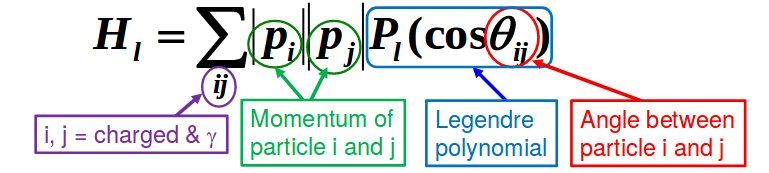
\includegraphics[width=7cm]{r2_v3.png}
\end{figure}

\vspace{-0.4 in}
\begin{columns}
	\column{0.5\textwidth}
	\begin{figure}
		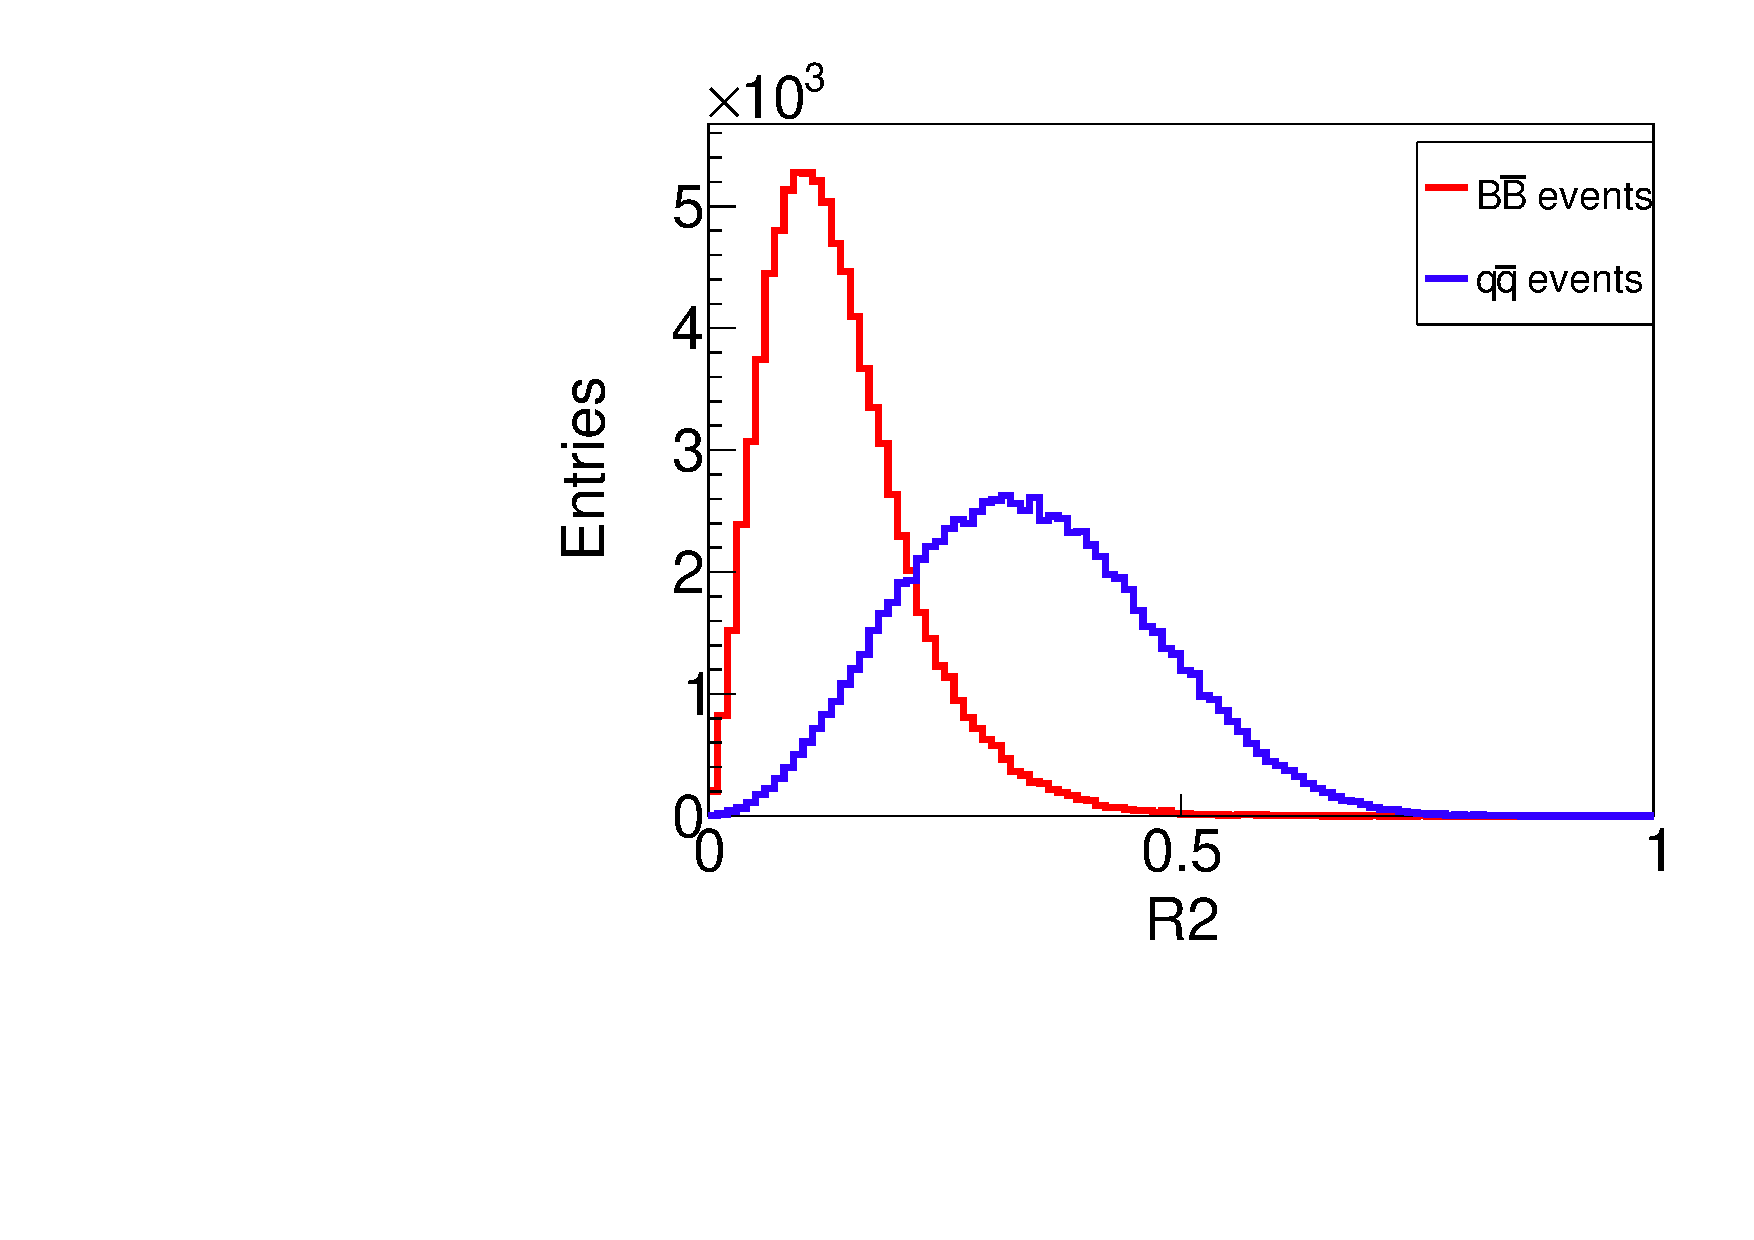
\includegraphics[width = 6cm]{R2.pdf}
	\end{figure}
	
	\column{0.5\textwidth}
	\begin{figure}
		\begin{tabular}{ c c}
			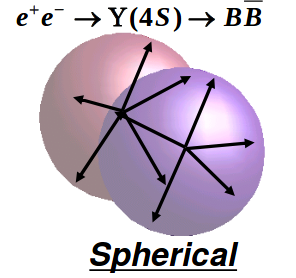
\includegraphics[height = 2.5 cm, width = 2.5cm]{cs2.png} &
			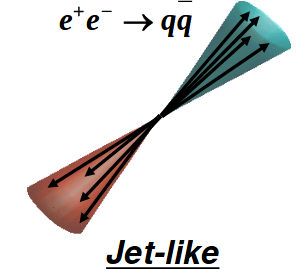
\includegraphics[height = 2.5 cm, width = 2.5cm]{cs3.png}\\[0.5ex]
		\end{tabular}
		\vspace{-0.2 in}
		%\caption{\tiny{Event topology: $ B\bar{B} $ (left) and $ q\bar{q} $ (right)}}
	\end{figure}
	
	\begin{itemize}
		\begin{scriptsize}
			\item Spherical limit: {\color{red}{$R_2 \rightarrow $ 0}}; jet-like limit: {\color{blue}{$R_2 \rightarrow $ 1}}.
			\item So we are on $ \Upsilon(4S) $ resonance and recording $ B\bar{B} $ pairs.
		\end{scriptsize}
	\end{itemize}
	
\end{columns}
\end{frame}


\begin{frame}[t]{R2}

			\begin{columns}
			\column{0.7\textwidth}
				\begin{figure}
				\vspace{-1cm}
				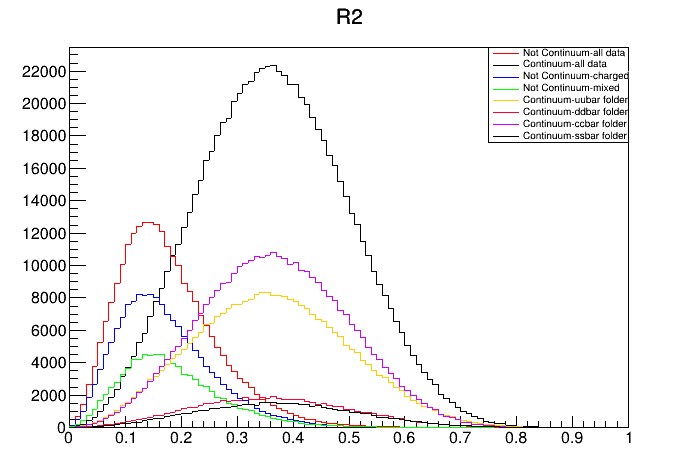
\includegraphics[height = 6 cm, width = 7.5cm]{R2_all.png}
				\caption{Plotting R2 for different set}
				\end{figure}			
			\column{0.3\textwidth}
			\begin{figure}
				\vspace{-0.8cm}
				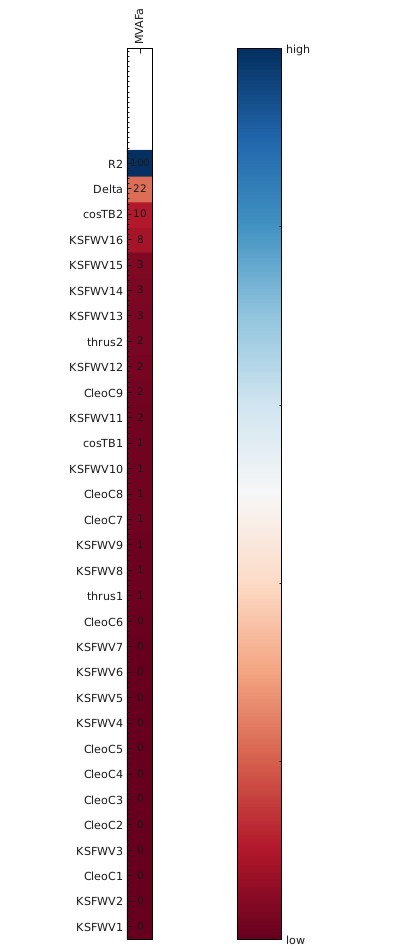
\includegraphics[height = 7 cm, width = 4cm]{importance.png}
				%\vspace{-0.8cm}
				%\fontsize{5pt}{5pt}\selectfont
				%\hspace{length}
				%\caption{Importance of different variables to predict continuum event}
			\end{figure}
		\end{columns}

\end{frame}

\begin{frame}[t]{FBDT output of R2 variable}

	\vspace{-0.3cm}
			%\begin{figure}
				\hspace{-0.1cm} 
				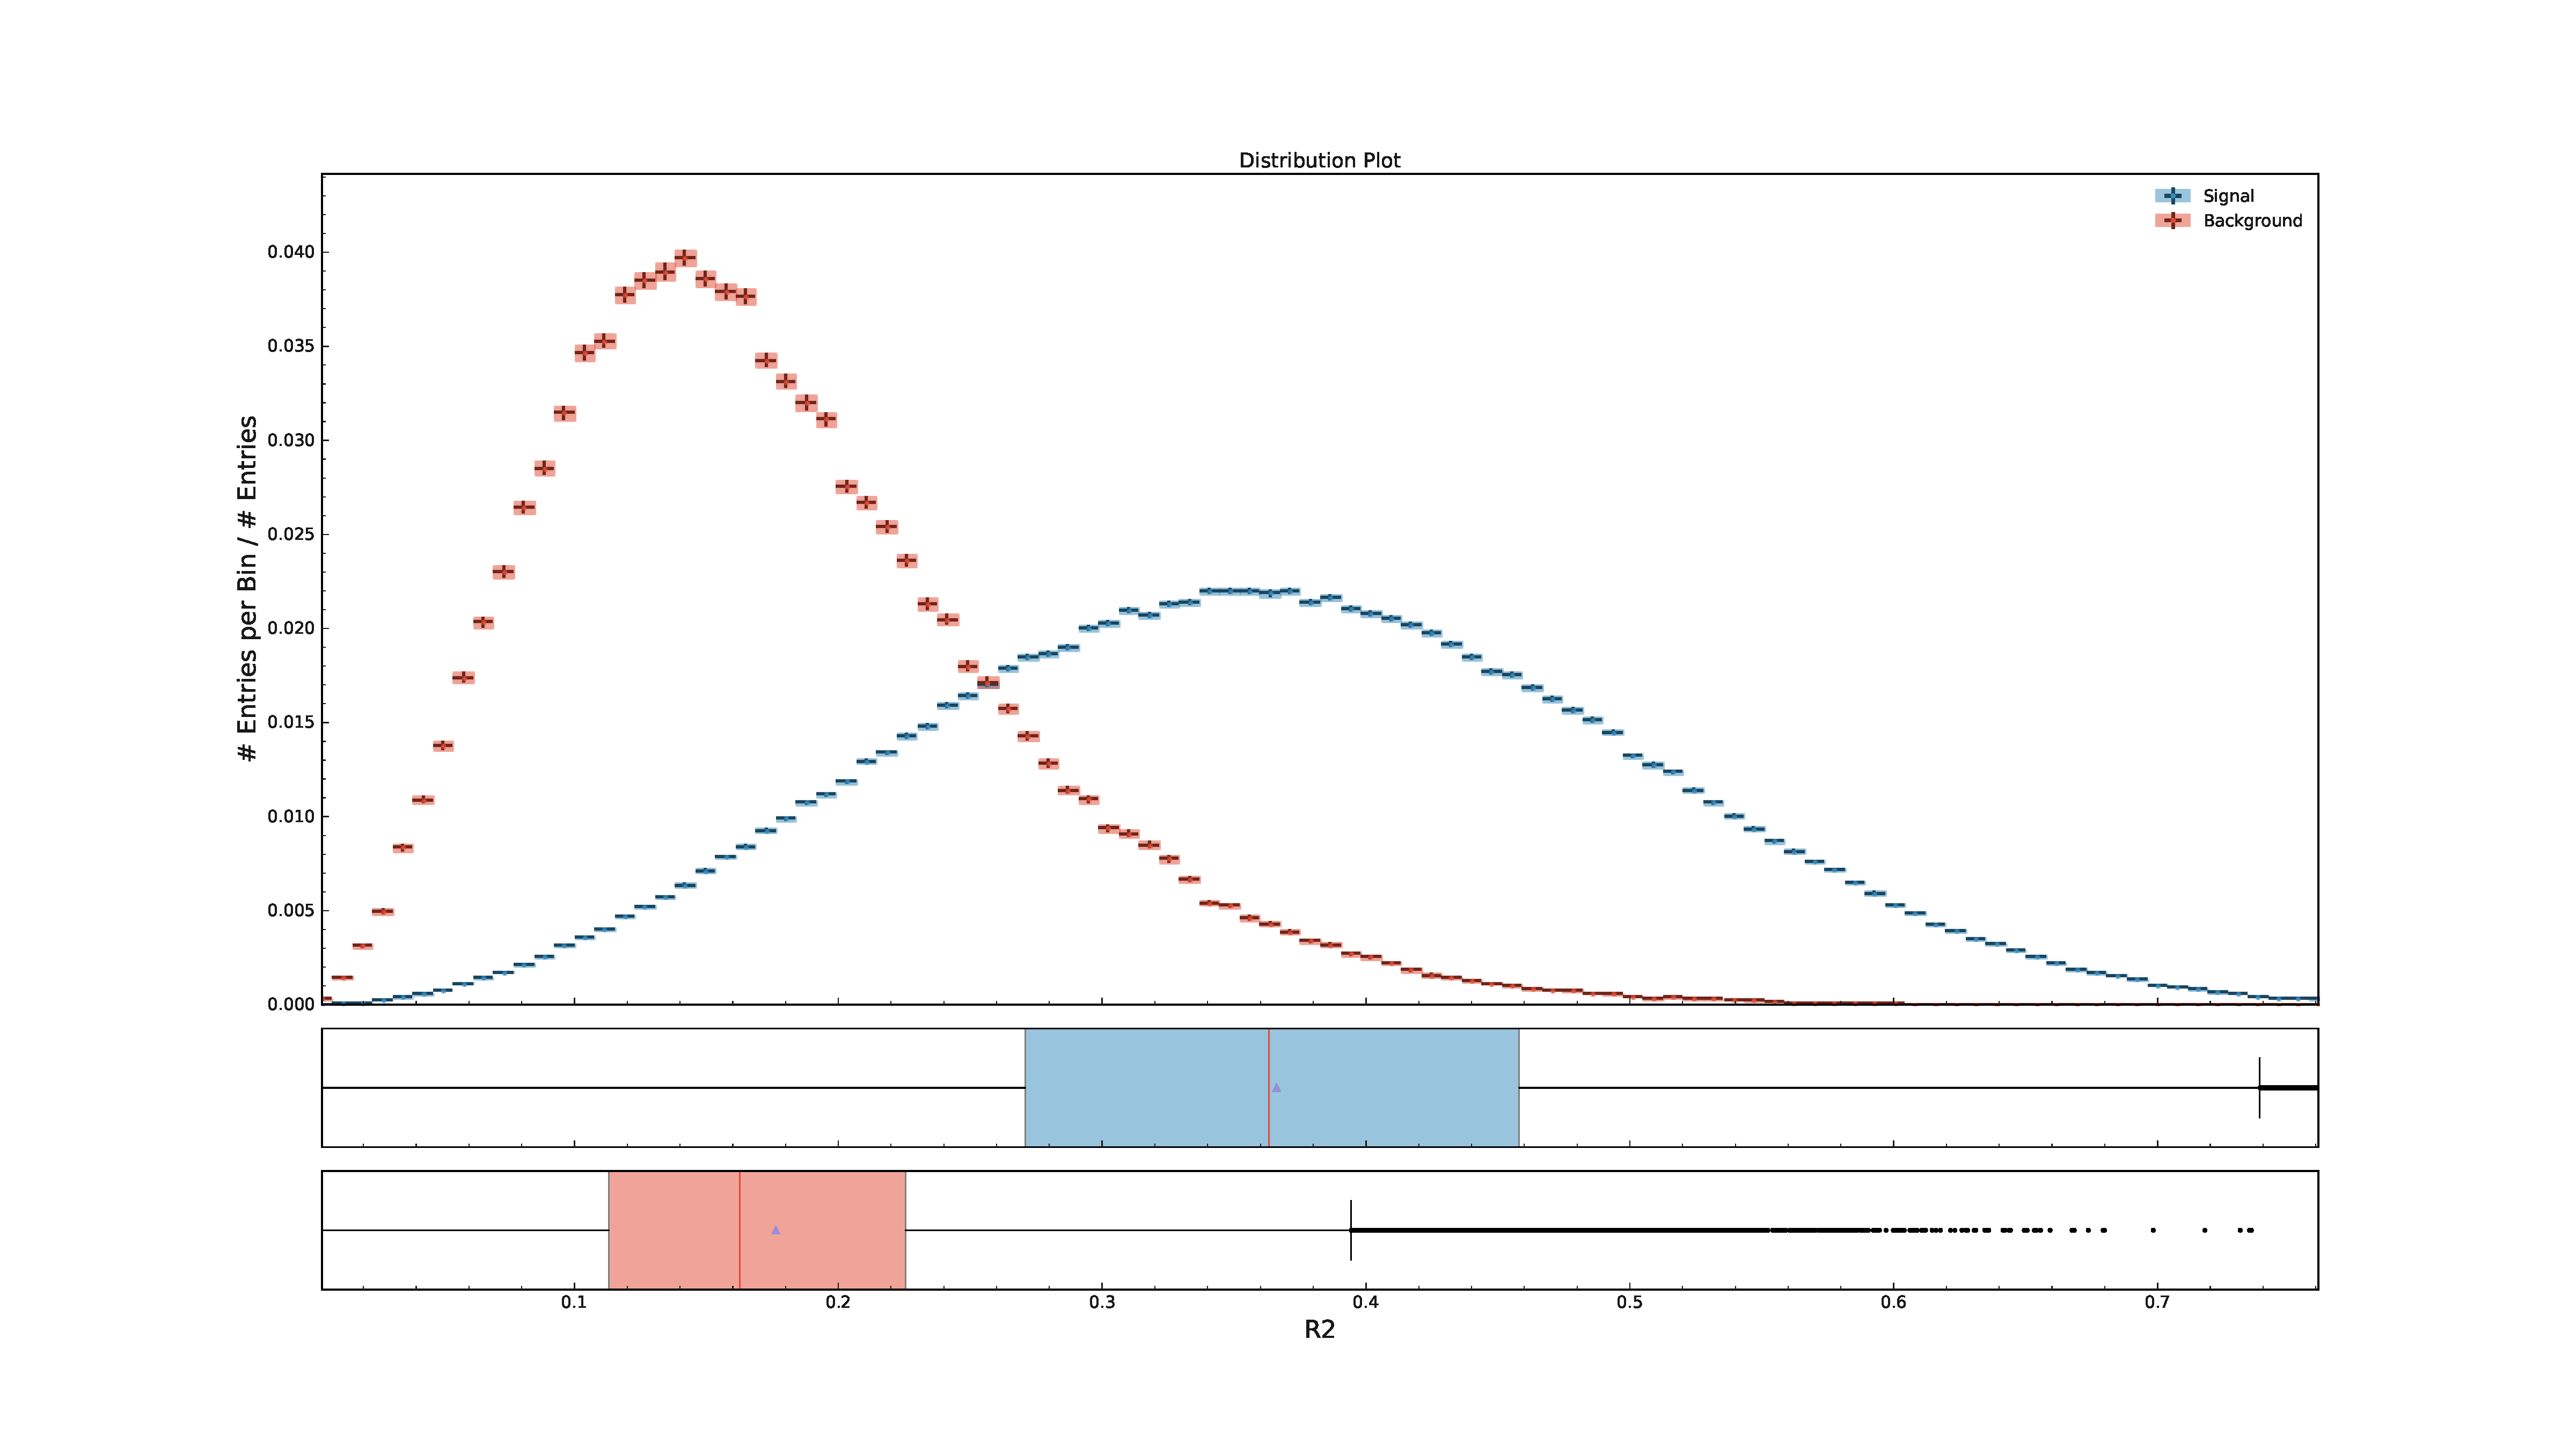
\includegraphics[height = 6 cm, width = 9.5cm]{bdt_r2.pdf}
				%\caption{MVC algorithm with Hierarchal approach}
			%\end{figure}
	\begin{scriptsize}
		\vspace{-0.6cm}
		\begin{itemize}
			\item Future plan:

				%\vspace{-0.5cm}
				\begin{itemize}
								\begin{scriptsize}
					\item Train FBDT in various way to get better cuts for continuum suppression.
					\item Finding all B$\bar{\rm B}$ mesons using Hadronic and Semileptonic tag in FEI.
								\end{scriptsize}
				\end{itemize}

		\end{itemize}
	\end{scriptsize}
\end{frame}

%--------------------------------------------------------------------------
%\section{References}
%--------------------------------------------------------------------------

%\begin{frame}[t, allowframebreaks]{References}
%	
%\scriptsize
%\begin{thebibliography}{9}
%	\bibitem{allen13} Allen, Theresa M. and Pieter R. Cullis. Liposomal drug delivery systems: from concept to clinical applications, \emph{Adv. drug del. Rev.}, 65(2013)36--48.
%	
%	\bibitem{saffman} Saffman P. G. and Taylor G., The penetration of a fluid into a medium of Hele-Shaw c58ell containing a more viscous liquid, \emph{Proc. Soc. London, Ser A}, 245(1958)312-329.
%	
%	\bibitem{sopan13} Sunthar, P. and Phappal, S. M.,  Influence of micro-mixing on the size of liposomes self-assembled from miscible liquid phases. \emph{Chem. phys. lipids}, 172-173(2013)20-30.
%	
%\end{thebibliography}	

%\bibliographystyle{apalike}
%\bibliography{mybib}
	
%\end{frame}


%--------------------------------------------------------------------------
\appendix
%--------------------------------------------------------------------------
\begin{frame}{Reference}
	\begin{scriptsize}
		\begin{itemize}
			\item The Belle II Physics Book (KEK Preprint 2018-27)
			\item The Physics of the B Factories (KEK Preprint 2014-3)
			\item Observables for the Analysis of Event Shapes in e$^{+}$e$^{-}$ Annihilation and Othere Processes (1978)(7811220, CALT-688680)
			\item Belle II Software Documentation$\rightarrow$ \href{http://software.belle2.org}{software.belle2.org}
			\item Root Data Analysis Framework user Guide$\rightarrow$ \href{https://root.cern/}{https://root.cern/}
		\end{itemize}
	\end{scriptsize}
\end{frame}

\begin{frame}{}                                                                           
	
\includegraphics[scale=0.6]{thankyou}
\end{frame}


\begin{frame}{}                                                                           

\end{frame}
\begin{frame}{}                                                                           
\end{frame}

\end{document}
